\chapter{Receptive field properties of the tree shrew superior colliculus neurons} 
\pagebreak
\section{Abstract}

	Though theories of orientation selectivity suggest that the sharp orientation selectivity observed in visual cortical neurons is developed for the first time in the primary visual cortex (V1), studies have shown that neurons in sub-cortical structures, especially the retina and the lateral geniculate nucleus (LGN), are tuned to orientation at higher spatial frequencies. If orientation selectivity arises from the retina, it should be evident in other targets of retinal projections. The superior colliculus (SC) is one such area. Here, I examined the orientation selectivity of SC neurons in tree shrews using thin bars and gratings of various spatial frequencies. I found that SC neurons show orientation tuning comparable to that observed layer 4 of V1 in the tree shrews and orientation biases reported in the retina and the LGN of cats and macaques. This orientation selectivity was more evident at higher spatial frequencies. These results indicate that orientation tuning observed in the inputs to the cortex maybe generated from the orientation biases present in earlier visual areas.
	
\pagebreak

\section{Introduction}

	The most prominent theory of orientation selectivity suggests that orientation tuning is generated for the first time in the primary visual cortex. The theory of excitatory convergence suggests that orientation tuning in the primary visual cortex is derived from inputs from circular lateral geniculate nucleus neurons that are arranged in a row converging on the V1 neuron. This theory has been widely contested with studies giving evidence for and against the theory. One belief that has been preserved is that orientation selectivity is generated in V1. This is supported by intracellular studies which show that inputs to the cortex are already tuned to orientation, a finding congruent with converging inputs. An alternate reason may be that orientation biases are already present in the subcortical areas which get sharpened by mechanisms such as thresholding and inhibition.
	
	Beginning in the early 70s, a long list of studies have shown that orientation tuning is present in sub cortical structures. Levick and Thibos (1980) initially showed that retinal ganglion cells were tuned to orientation at higher spatial frequencies. This observation has since been confirmed in both cats and macaques at the level of the retina and the LGN. The retinal orientation biases are set to be derived from the natural growth pattern of the retina which elongates the dendritic fields. Given that orientation tuning is only observed at higher spatial frequencies and the fact that V1 neurons only respond at higher spatial frequencies, the degree of orientation tuning observed in the inputs to V1 can be generated by a mere sharpening of biased inputs. 
	
	Both the theories discussed above could be a possible explanation for the orientation tuning observed in the inputs to the cortex are tuned to orientation. However, if the retina were the seed of orientation selectivity in the visual system, then orientation tuning should be seen in other regions of the brain that receive inputs from the retina. For a long time, evidence suggested that this was not the case. One area of the brain that receives input from the retina is the superior colliculus. The superior colliculus in cats and macaques prominently show no orientation biases. However, recent studies have shown that rodent SC has orientation tuned neurons. We believe that this is because orientation tuning in subcortical areas are only present at higher spatial frequencies and studies that looked for orientation tuning in the SC did not take this into account. Here we looked for orientation biases in the tree shrew superior colliculus.
	
	The tree shrew was chosen for a few important reasons, foremost of which is that it has a large, distinctly laminated superior colliculus. Studies show that as in macaques and cats, the superficial layers of the shrew SC receives direct input from the retina and has been implicated in form discrimination. These layers are also part of an independent pathway to the extrastriate cortex which is essential in form perception. However, unlike cats and macaques, the tree shrew superior colliculus is easy to record from and a previous study showed that a small proportion of neurons in the superficial layers of the shrew SC had distinctly elongated fields. This particular study might have missed any small orientation biases, similar in extent to the retina as they only reported fields that were 3 or more times longer than they were wide. Rodent models were excluded as the mechanism through which orientation selectivity is derived in rodents is considered to be to the mechanism in other mammals that have been studied.
		
	Here orientation bias in the superior colliculus of the tree shrew was examined in an attempt to show that orientation tuning in the inputs to the cortex was a reflection of the bias observed in the retina. We hypothesised that orientation tuning will be revealed in the superior colliculus at higher spatial frequencies. In particular:
	a) When using thin, moving bars, the neurons will be tuned to orientation and;
	b) When tested using gratings of different spatial frequencies and orientation, there would be orienation tuned response at higher spatial frequencies compared to those at lower spatial frequencies.


	

\section{Methods}
	\subsection{Isolating Superior Colliculus and Electrophysiology}
		The superior colliculus in the tree shrew is large and well laminated structure and runs from the posterior edge of the brain to AP 2. Following surgery, a craniotomy was performed over the location of the superior colliculus. High impedence tungsten microelectrodes were lowered into the brain and the signal was amplified and filtered and fed into an audio speaker as well as an analog to digital converter and recorded. The SC was identified by listening to the neuronal activity in the speaker. The data was recorded as a spike trace using the spike 2 software. The spikes were templated and the spike timing exported as a text file. Further analysis was performed using custom MATLAB code.
		
	\subsection{Stimuli}
	
		Stimuli was presented using a Barco monitor and the stimuli were generated using Visage (VSG). For each SC neuron, the preferred orientation was measured using a thin bar sweeping bi-directionally (Check if there is a particular size of the bar that we preferred). Then, the spatial frequency response to a gratings of different orientations was also measured.
		
	\subsection{Data Analysis}
		
		As mentioned in section 3 (Methods), Spike Density Functions were constructed for both the bar and gratings. For orientation tuning recorded using a bar, the maximum response for each orientation was plotted on a polar diagram. The circular mean of the angular response was considered the optimum orientation. The circular variance was calculated as a measure of sharpness of the orientation tuning.
		
		For the gratings, the FFT of the spike density function was calculated. Then the F0/F1 ratio was calculated. If the ratio was less than 1, the cell was deemed to be X- like and the F1 component of the repsonse was used for further analysis. If the ratio was greater than 1, the cell was considered non-linear and the F0 component was used.
		
		The bandwidth during which the superior colliculus neurons responded for the optimum orientation but not for the orthogonal orientation was calculated. In order to do this,  a minimum response was first defined as the response rate at the spatial frequency where the response between the optimum and orthogonal orientations were not significantly different. The SF bandwidth was then the difference between the SF when the response for the orthogonal orientation reached the minimum response and the SF where the optimum orientation resposne reached the minimum resposne.
		
\section{Results}
	\subsection{Anatomical location of units}

		Using the histological reconstructions described in methods, the laminar position of 21 units from three Tree Shrews was determined. The results are presented in Figure 6.1. The reconstruction shows that most neurons were present in the Stratum Griseum Superficiale (SGS) where the majority of retinal inputs terminate.
			\begin{figure}
			
				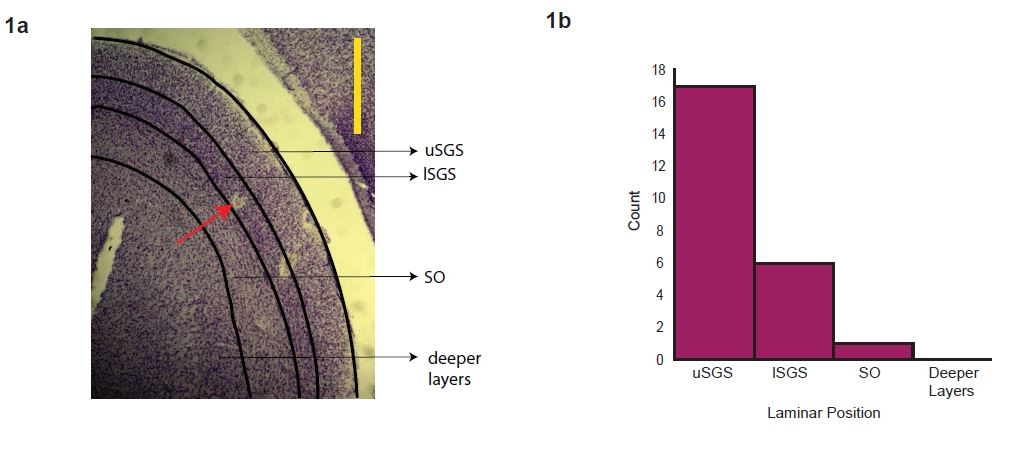
\includegraphics[width=\linewidth]{SCLaminarPosition.jpg}
				\caption{Histology. a) A section of tree shrew superior colliculus showing electrolytic lesions. Red arrow
					points to an electrolytic lesion. Scale bar (yellow vertical line) denotes 1000 μm. b) A summary of laminar
					position of recorded units in the superior colliculus. Abbreviations: uSGS- upper Stratum Griseum Superficiale;
					lSGS- lower Stratum Griseum Superficiale; SO- Stratum Opticum.}
				\label{fig:fig1}
			\end{figure}
			
		
			
	\subsection{Orientation Selectivity}
		
		The responses of a representative neuron to thin bars of changing orientation are presented in figure 6.2. The response shown in the figure is the average spike rate of the neuron over 10 trials. The corresponding orientation tuning curve along with the orientation tuning curves of our most and least tuned neurons are presented in the figure below. 
		
			\begin{figure}
				
				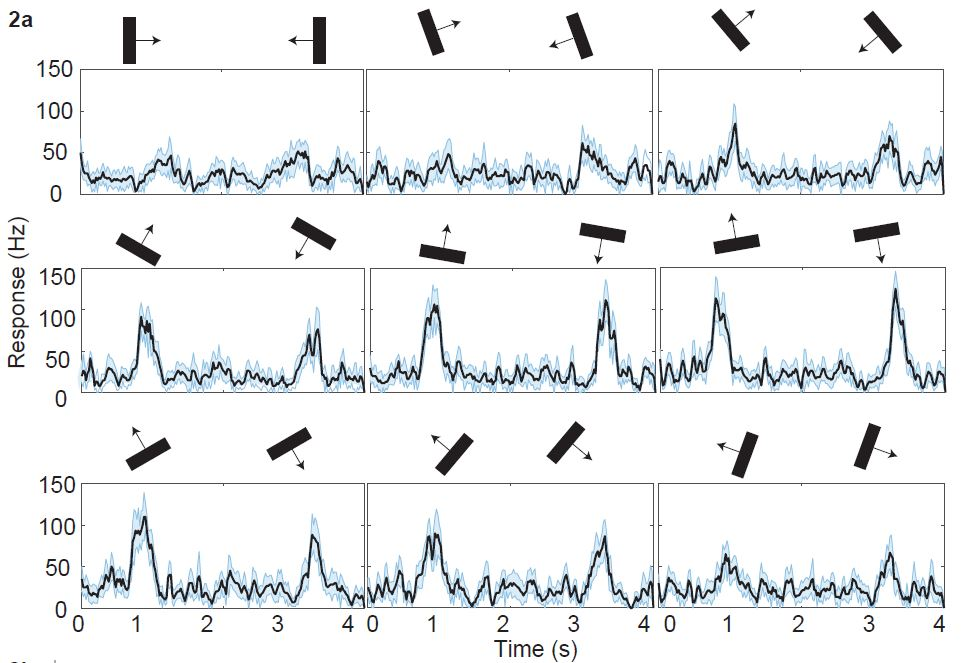
\includegraphics[width=\linewidth]{SCOriResp.jpg}
				\caption{Orientation response of an example cell.
					2a) Spike density functions (20 ms bins smoothed over
					3 bins) of the neuron’s response to oriented bar (direction
					of motion above each peak).}
				\label{fig:fig2}
			\end{figure}
			
		
			\begin{figure}
				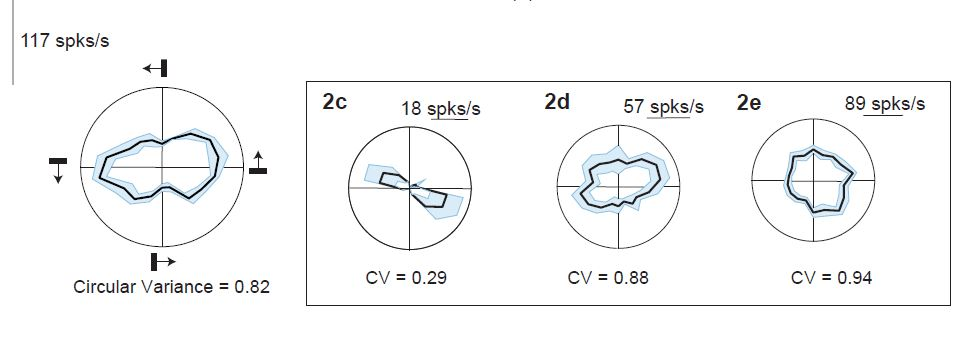
\includegraphics[width=\linewidth]{SCOriTuning.jpg}
				\caption{Polar plot showing
					the orientation tuning of the bar. Error bars denote
					Standard error. Orientation tuning curves of the
					sharpest (2c) and the least tuned (2d) neurons
					included in our analysis. (2e) was the least tuned
					neuron in our sample}
				\label{fig:fig3}			
			\end{figure}
		
		The circular variance was calculated as described earlier to indicate the degree of orientation tuning demonstrated by the neurons studied. Any neuron that had a CV of greater that 0.9 was said to be non-oriented for the purposes of this study. The median CV we observed was 0.82 with a range of [0.21, 0.94]. Two neurons which had a CV of greater than 21 were excluded from further analysis. A distribution of the circular variances is presented below.
			\begin{figure}
				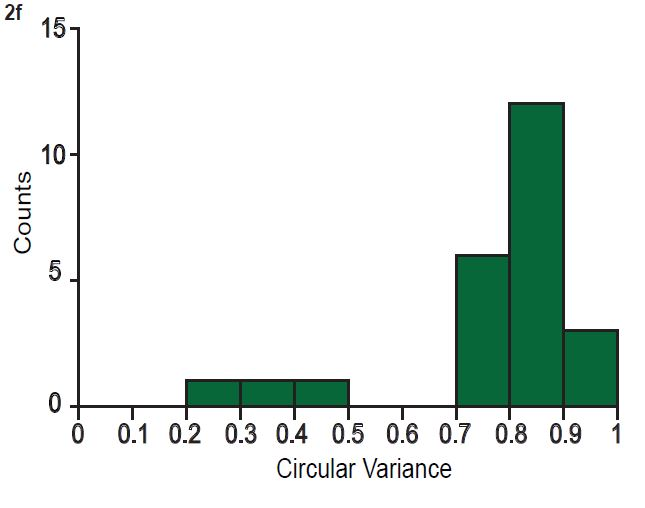
\includegraphics[width=\linewidth]{SCCircVar.jpg}
				\caption{This figure demonstrates the distribution of circular
					variances of all neurons.}
				\label{fig:fig4}			
			\end{figure}
		
		
		
	\subsection{Spatial Frequency Tuning}
		The spatial frequency response of the neurons were also tested in relation to different orientations. The difference in response between the optimum and non-optimum orientation was calculated as described in the methods. We found that on average, the response to the orthogonal orientation reached the minimum 0.5 cpd before the response to the optimum orientation; with the 95 percent CT= [0.4, 0.6] ]
		
			\begin{figure}
				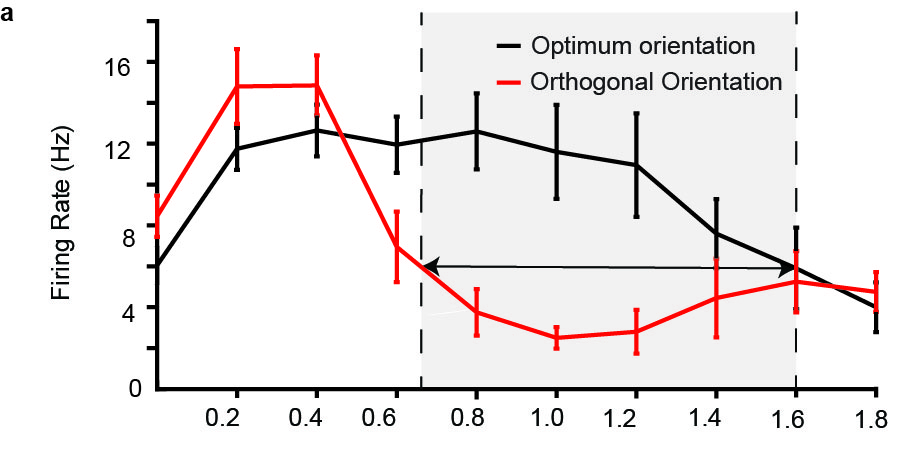
\includegraphics[width=\linewidth]{SCOptOrth.jpg}
				\caption{Example SF tuning curves for optimal and orthogonal orientations. The cut-off frequency at the
					optimal orientation is the SF at which the response at optimal orientation is no longer significantly different from the response at orthogonal
					orientation. The response at the cut-off frequency for optimum orientation is called the minimum response. For the orthogonal orientation, the
					cut-off frequency was the SF at which minimum response was first reached.}
				\label{fig:fig5}			
			\end{figure}

			\begin{figure}
				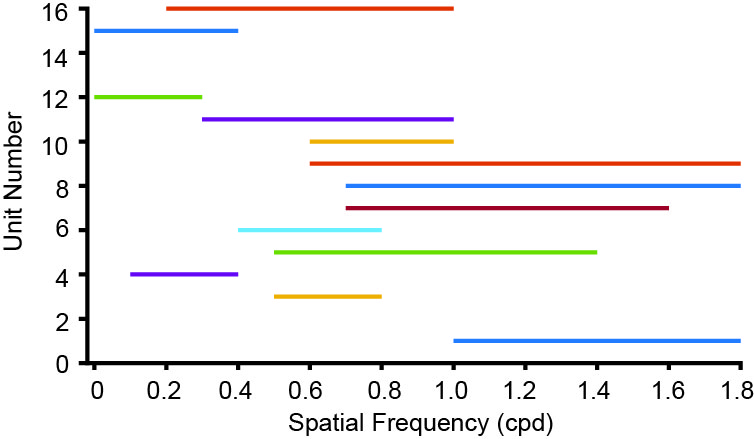
\includegraphics[width=\linewidth]{SCSFTuning.jpg}
				\caption{ The difference between the cut-off frequencies for the optimum
					and orthogonal orientations for 16 units is shown in Figure 3b.}
				\label{fig:fig6}			
			\end{figure}
\section{Discussion}

Results show that superior colliculus neurons are tuned to orientation at higher spatial frequencies. I postulated that if the orientation tuning observed in the inputs to the cortex indeed originated in the retina rather than through the convergence of unbiased geniculate inputs, then if orientation tuning is measured along a pathway other than the geniculo-striate pathway, orientation biases similar to that observed in the retina would be found in the superior colliculus, which is in an alternative pathway. That is, when tested with thin bars, the SC neurons will be orientation selective and when tested with grating stimuli, the orientation tuning would be predominantly observed at higher spatial frequencies. These findings are comparable to  Our results are congruent with this finding suggesting that orientation tuning in the primary visual cortex originates from biases in the retina. 



\subsection{Anatomical Relevance}

What did you find?
Orientaiton bias in the superior colliculus at higher spatial frequencies.
So what?
well orientation bias is in the retina.
Ok?
And everyone thinks that orientation selectivity is generated in the cortex.
So what does this show?
It shows that orientation selectivity is present earlier in the visual system. 
Is this the first time that's been shown?
No. It's been shown in the LGN and in the retina.
OK? So what's new?
Reporting orientation bias in the superior colliculus means that orientation bias is probably inherited from the retina.
So what?
Being present earlier in the visual system means that the visual system doesn't have to reinvent the wheel over and over again.

\subsection{Orientation selectivity in shrew superior colliculus}
\subsection{Direction selectivity}
\subsection{Similarities and differences with other species}


